\problemname{Bokstavstärningar}

Klara har $N$ bokstavstärningar.
Varje tärning har en bokstav på var och en av sina $2 \le K \le 20$ sidor.
Genom att slå tärningarna och ordna dem på valfritt sätt kan man skapa ett ord med $N$ bokstäver.

Skriv ett program som räknar ut hur många giltiga ord man kan skriva med Klaras bokstavstärningar.
Till din hjälp har du en ordlista som innehåller alla $M$ giltiga ord med $N$ bokstäver.

\begin{figure}[ht!]
\centering
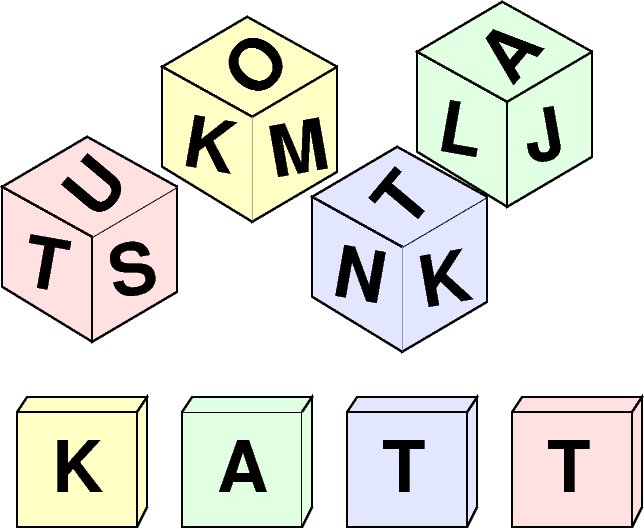
\includegraphics[width=0.6\textwidth]{tarningar.png}
\caption{En illustration av det första exemplet. Eftersom $K=3$ innehåller endast tre sidor på tärningarna bokstäver. Det går också att skriva STOL, men inte NATT.}
\label{overflow}
\end{figure}

\section*{Input}

Den första raden i indatan innehåller tre heltal: $N$, $K$ och $M$.
Därefter följer $N$ rader med vardera $K$ bokstäver, bokstäverna på varje tärning.
Sist kommer $M$ rader med vardera $N$ bokstäver, listan på alla giltiga ord.

Enbart stora engelska bokstäver (A-Z) förekommer i indata.

Ingen bokstav kan förekomma på mer än en sida av en tärning.

\section*{Output}

Ditt program ska skriva ut ett enda heltal: antalet giltiga ord som kan skrivas.

\section*{Poängsättning}
Din lösning kommer att testas på en mängd testfallsgrupper. För att få poäng för en grupp så måste du klara alla testfall i gruppen.

\begin{tabular}{| l | l | l |}
	\hline
	Grupp & Poängvärde & Begränsningar\\ \hline
	1     & 9          & $K = 2, N \le 4, M \le 100$ \\ \hline
	2     & 9          & $K \le 6, N \le 5, M \le 100$ \\ \hline
	3     & 12         & $K \le 20, N \le 6, M \le 1000$ \\ \hline
	4     & 14         & $K \le 15, N \le 6, M \le 10\,000$ \\ \hline
	5     & 21         & $K \le 20, N \le 6, M \le 100\,000$ \\ \hline
	6     & 35         & $K \le 10, N \le 15, M \le 500$ \\ \hline
\end{tabular}
